The area of a parallelogram is defined as
\begin{align}
\norm{\vec{a} \times \vec{b}}
\end{align}
where
\begin{align}
\vec{a} \times \vec{b} = 
\myvec{
      0       & -a_3    & a_2 \\ 
      a_3       & 0    & -a_1 \\
      -a_2       & a_1     & 0 
}      
\myvec{
      b_1 \\ 
      b_2 \\
      b_3 
}
\\
=\myvec{
      0       & -4    & 1 \\ 
      4       & 0    & -3 \\
      -1       & 3     & 0 
}
\myvec{      
      1\\ 
      -1\\
      1
}      
=\myvec{
      5\\ 
      1\\
      -4
}      
\end{align}
Thus, the desired area is 
\begin{align}
\norm{\vec{a} \times \vec{b}} = \sqrt{5^2 + 1^2 + (-1)^2}
\\
=3\sqrt{3}
\end{align}
The  following Python code generates Fig. \ref{fig:solutions_quad_8paral_sss_py}
%
\begin{lstlisting}
codes/parallelogram.py
\end{lstlisting}
\begin{figure}[!ht]
\centering
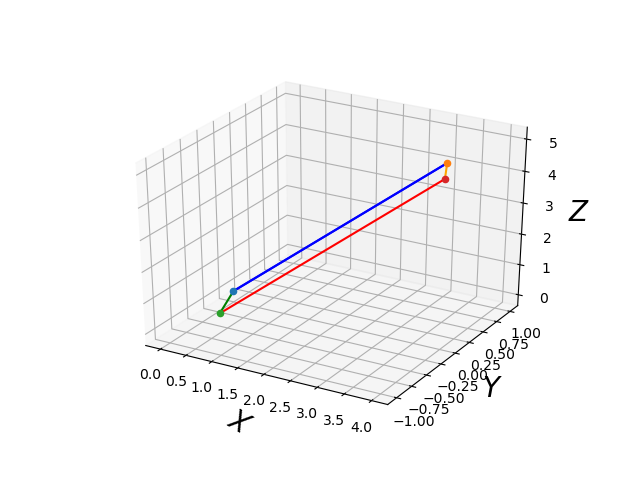
\includegraphics[width=\columnwidth]{./solutions/quad/8/figs/parallelogram.png}
\caption{Parallelogram generated using python 3D-plot}
\label{fig:solutions_quad_8paral_sss_py}
\end{figure}

The  following Python code verifies the cross-product value.

\begin{lstlisting}
codes/cross_product_check.py
\end{lstlisting}
